% !TEX root = ../Seminararbeit-Data_Mining_Frameworks.tex
%


% =============================================================================
%
% Der Data Mining Prozess
%
% =============================================================================
\chapter{Der Data Mining Prozess}
\label{sec:process}

Der Prozess des Data Minings lässt sich grundsätzlich durch die folgenden Phasen
beschreiben:
\begin{enumerate}
\item Sammeln von Daten: \\
Für das Sammeln von Daten ist unter Umständen spezielle Hardware, bspw.
Sensoren, händische Arbeit wie das Sammeln von Umfragebögen oder Software in
Form einer Webanwendung mit auszufüllenden Formularfeldern, notwendig. Auch wenn
diese Phase sehr Anwendungsspezifisch ist und oft vom Daten-Analysten nicht
beeinflusst werden kann, ist sie ausschlaggebend für das Ergebnis des Data
Mining Prozesses.
\item Bereinigen der Daten: \\
Oftmals sind die gesammelten Rohdaten aufgrund des Dateiformats oder einer
fehlenden Struktur nicht direkt verarbeitbar. Deshalb ist es wichtig, die Daten
in ein Format zu bringen, welches von Data Mining Algorithmen gelesen werden
kann.
\item Analyse der Daten: \\
Der letzte Schritt ist die Daten analytisch zu verarbeiten und Methoden zu
entwickeln, um diese nutzbar zu machen. Dies geschieht durch das Anwenden von
bestimmten Data Mining Algorithmen, welche für die jeweilige Aufgabenstellung
angepasst werden müssen.
\end{enumerate}
Um einen Standard für einen solchen Data Mining Vorgang zu etablieren, haben
einige große Unternehmen wie Automobilhersteller Daimler-Benz, Versicherungs
Provider OHRA, Hard- und Software Hersteller NCR Corp. und Statistik-Software
Hersteller SPSS Inc. den „CRoss-Industry Standard Process for Data Mining“
(kurz: CRISP-DM) definiert.

\pagebreak

\section{CRISP-DM}
\label{sec:process:crispdm}

\begin{figure}[htb]
	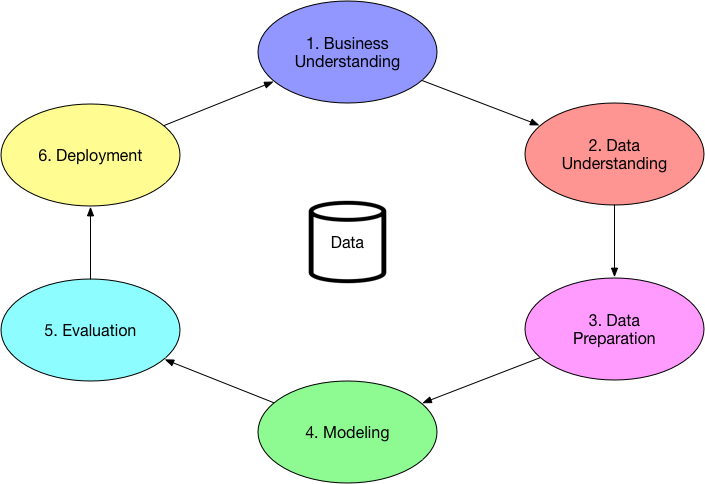
\includegraphics[width=\textwidth]{gfx/CRISP-DM_Model.png}
	\caption{Konzeptionelles CRISP-DM Modell}
	\label{fig:process:crispdm}
\end{figure}



\subsection{Business Understanding}
\label{sec:process:crispdm:bu}

Im ersten Schritt des CRISP-DM Prozesses, dem sog. Business- (oder auch Organizational) Understanding,
ist es zunächst wichtig festzulegen was man mit dem Minen von Daten erreichen
möchte bzw. welche Informationen von Interesse sind. Hier findet auch eine oft
zitierte Textstelle aus Alice im Wunderland Anwendung:
\begin{quotation}
  >>Willst du mir wohl sagen, wenn ich bitten darf, welchen Weg ich hier nehmen muß?<< \\
  >>Das hängt zum guten Teil davon ab, wohin du gehen willst,<< sagte die Katze. \\
  >>Es kommt mir nicht darauf an, wohin –<< sagte Alice. \\
  >>Dann kommt es auch nicht darauf an, welchen Weg du nimmst,<< sagte die Katze. \\
  >>– wenn ich nur irgendwo hinkomme,<< fügte Alice als Erklärung hinzu. \\
  >>O, das wirst du ganz gewiß,« sagte die Katze, »wenn du nur lange genug gehest.<<
\end{quotation}
In Bezug auf das Thema Data Mining bedeutet das, dass es keine Rolle spielt wie
lange man Daten Mined, wenn
man nicht definiert hat welche Informationen man gerne hätte. Es müssen also
zunächst Fragen festgelegt werden, welche durch das Data Mining beantwortet
werden sollen. Beispielsweise möchte man gerne wissen warum sich Kunden so sehr
beschweren, wie man die Profit-Spanne seiner Produkte vergrößert oder wie man
Fehler bei der Herstellung antizipieren kann.

\subsection{Data Understanding}
\label{sec:process:crispdm:du}

Man muss zunächst zwischen zwei Systemen unterscheiden.
\begin{itemize}
  \item OLTP - Online Transaction Processing System: \\
  Als OLTP werden die meisten relationalen Datenbank Systeme bezeichnet. Sie
  sind ausgelegt für eine große Anzahl an „Reads“ und „Writes“. Ein Beispiel
  hierfür ist der Kassiervorgang im Supermarkt, bei dem in einer kurzen Zeit
  viele Gegenstände per Barcode registriert werden müssen. Diese Systeme sind
  durch die Normalisierung nicht besonders für die Analyse geeignet, da mitunter
  sehr viele Joins ausgeführt werden müssen.
  \item OLAP - Online Analytical Processing System:
 \\
  Hat man die Daten in Form eines Data Warehouses in denormalisierter Form
  vorliegen, spricht man von einem OLAP. Wie der Name schon verrät eignen sich
  diese Datenbank Systeme zur Analyse der Daten, da hier die Datensätze zu einer
  geringen Zahl an Tabellen zusammengefasst wurden. Zu Beachten ist dabei
  allerdings, dass durch den Vorgang der Denormalisierung auch Redundanz
  auftritt und daher mehr Speicherplatz benötigt wird.
\end{itemize}

Schließlich muss man auch die Daten selbst unterscheiden. Hier existieren zwei
Typen mit welchen man Data Mining betreiben kann.
\begin{itemize}
  \item Operational Data:
 \\
  Diese Daten stammen aus Systemen, welche auf Transaktionen basieren. Dies
  können beispielsweise Daten aus Online-Bestellungen, Check-In Informationen am
  Flughafen oder anderen alltäglichen Aktivitäten sein. Allerdings sind diese
  Daten auch sehr detailliert und könnten daher unter Umständen die Privatsphäre
  verletzen.
  \item Organizational Data:
 \\
  Hierbei handelt es sich um Daten welche anonymisiert und zusammengefasst
  wurden. Dadurch wird sowohl die Privatsphäre des Einzelnen geschützt als auch
  die Möglichkeit geboten effizient Informationen wie bspw. Trends zu erkennen.
\end{itemize}

Wichtig ist hier die Zuverlässigkeit und Genauigkeit der Daten zu überprüfen,
denn Entscheidungen basierend auf ungenauen Daten sind auch entsprechend ungenau.

\subsection{Data Preparation}
\label{sec:process:crispdm:dp}

In diesem Schritt müssen die gesammelten Rohdaten verarbeitbar gemacht werden.
Beispielsweise müssen verfälschte bzw. für die Analyse unwichtige Daten
herausgefiltert, Attribute und deren Typen transformiert oder generell
Datensätze bereinigt werden. Letztendlich müssen die Daten so aufbereitet
werden, dass die Data Mining Algorithmen im nächsten Schritt damit arbeiten
können. Dies ist daher auch der aufwendigste Schritt im kompletten CRISP-DM
Prozess.

\subsection{Modeling}
\label{sec:process:crispdm:mod}

Die Data Mining Modelle kann man wiederum in 2 Arten unterteilen.
\begin{itemize}
  \item Deskriptive Modelle (engl.: „descriptive Model“): \\
  Diese Art von Modell trifft zwar keine Vorhersage über zukünftige Werte, kann
  aber Informationen über die immanente Struktur der Daten und Relationen
  liefern. Ein Beispiel hierfür ist die sog. Korrelationsmatrix
  \begin{figure}[htb]
    \centering
  	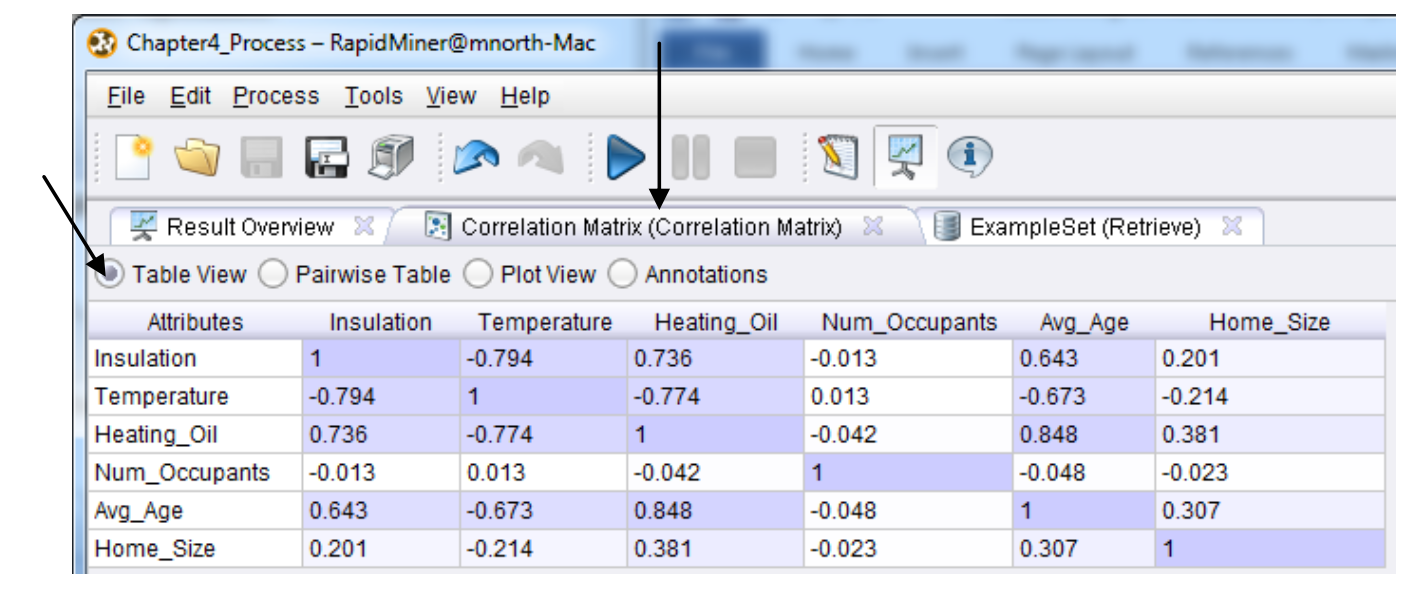
\includegraphics[width=0.5\textwidth]{gfx/correlationmatrix.png}
  	\caption{Ergebnis einer Korrelationsmatrix \cite{North:2012}}
  	\label{fig:process:crispdm:mod:cm}
  \end{figure}
  \\
  Korrelation bezeichnet eine statistische Aussage darüber wie stark Beziehungen
  zwischen Attributen in einem Datensatz sind.
  \item Vorhersagende Modelle (engl.: „predictive Model“): \\
  Wie sich anhand des Namens vermuten lässt, sagt ein vorhersagendes Modell
  einen bestimmten oder mehrere Werte voraus. Entscheidungsbäume (engl.: Decision
  Trees) sind ein Beispiel für ein solches vorhersagendes Modell.
  \pagebreak
  \begin{figure}[htb]
    \centering
  	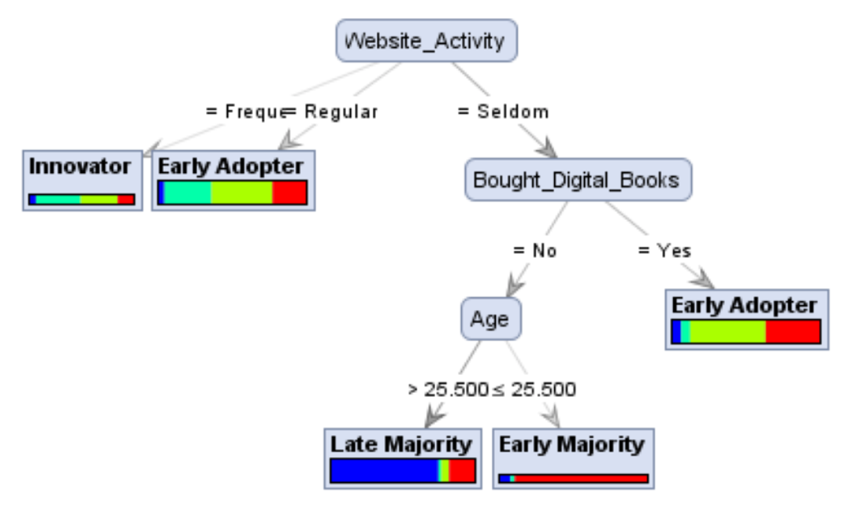
\includegraphics[width=0.5\textwidth]{gfx/dectree.png}
  	\caption{Ergebnis eines Entscheidungsbaums \cite{North:2012}}
  	\label{fig:process:crispdm:mod:dt}
  \end{figure}
  \\
  Entscheidungsbäume sind eine grafische Darstellung von  hierarchisch
  aufeinanderfolgenden Entscheidungen.
\end{itemize}
Prinzipiell versucht man beim Modeling ein Modell zu erschaffen (bzw. zu
„trainieren“), welches die echte Weit so gut wie möglich repräsentiert. Man tut
dies, um damit entweder fundierte Aussagen über die Zukunft treffen zu können
oder bisher unbekannte Informationen über den aktuellen Zustand zu erhalten.

\subsection{Evaluation}
\label{sec:process:crispdm:eval}

Hat man ein Modell trainiert und ein entsprechendes Ergebnis erhalten muss man
im nächsten Schritt prüfen, ob dieses auch sinnvoll ist. Analysen können, bspw.
aufgrund von falschen Parametern im Algorithmus oder durch ungenaue Daten,
fehlerhaft sein. Ist dies der Fall muss entweder das Modell entsprechend
angepasst werden bzw. die Daten im Schritt „Data Preparation“ weiter bearbeitet
werden. Außerdem muss das Ergebnis auf Relevanz und das Model somit auf
Aussagekraft geprüft werden. Basieren Ergebnisse auf einer geringen Anzahl an
Datensätzen, kann dies zu fälschlichen Annahmen bzw. unzutreffenden
Informationen führen.

\subsection{Deployment}
\label{sec:process:crispdm:depl}

Ist man mit seinem Modell und dessen Aussagekraft zufrieden, kann man den
Prozess automatisieren. Dies geschieht durch die Implementierung in ein
(wahrscheinlich bereits vorhandenes) Informationssystem. Außerdem kann man mit
den gewonnenen Informationen nun Entscheidungen treffen, wobei jedoch folgendes
beachtet werden muss: \\
Korrelation bedeutet nicht Kausalität! Nur weil, bspw. durch eine
Korrelationsmatrix, zwischen zwei Attributen eine Korrelation festgestellt
wurde, heißt das nicht, dass der Wert eines Attributs der Grund für einen Wert
des korrelierenden Attributs ist.

\section{Alternativen}
\label{sec:process:alt}

Die folgende Tabelle zeigt Umfrageergebnisse zu der Frage welche Methode für
die Analyse bzw. das Data Mining im Unternehmen der Befragten zum Einsatz komme.
Betrachtet man die Ergebnisse tauchen neben einigen spezifischen Prozessen auch
der sog. SEMMA Prozess und der KDD Prozess auf.

\begin{figure}[htb]
	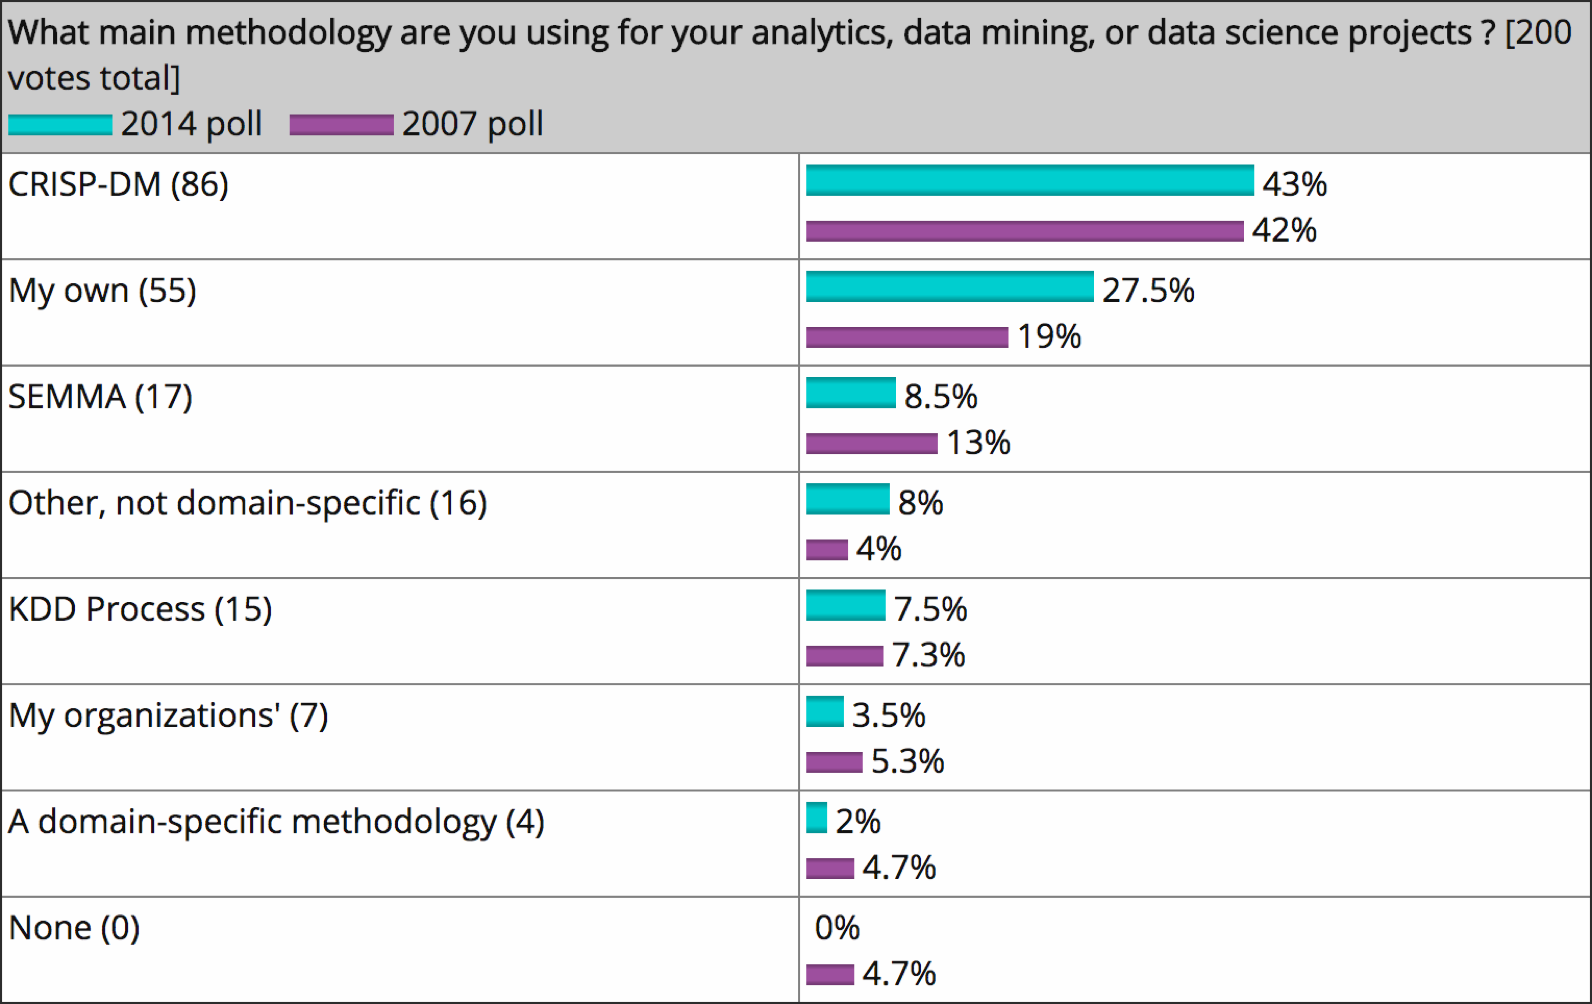
\includegraphics[width=\textwidth]{gfx/dmprocesses.png}
	\caption{Umfrage welche DM-Prozesse im Unternehmen zum Einsatz kommen \cite{KDN}}
	\label{fig:process:alt:cor}
\end{figure}

\subsection{Der Data Mining Prozess KDD}
\label{sec:process:alt:kdd}

In Fayyads „Knowledge Discovery in Databases“ \cite{FAY:96} wird Data Mining als
eine der Phasen des  Prozesses gesehen, welche zur „Gewinnung von Erkenntnissen“
dienen soll.

\begin{figure}[htb]
	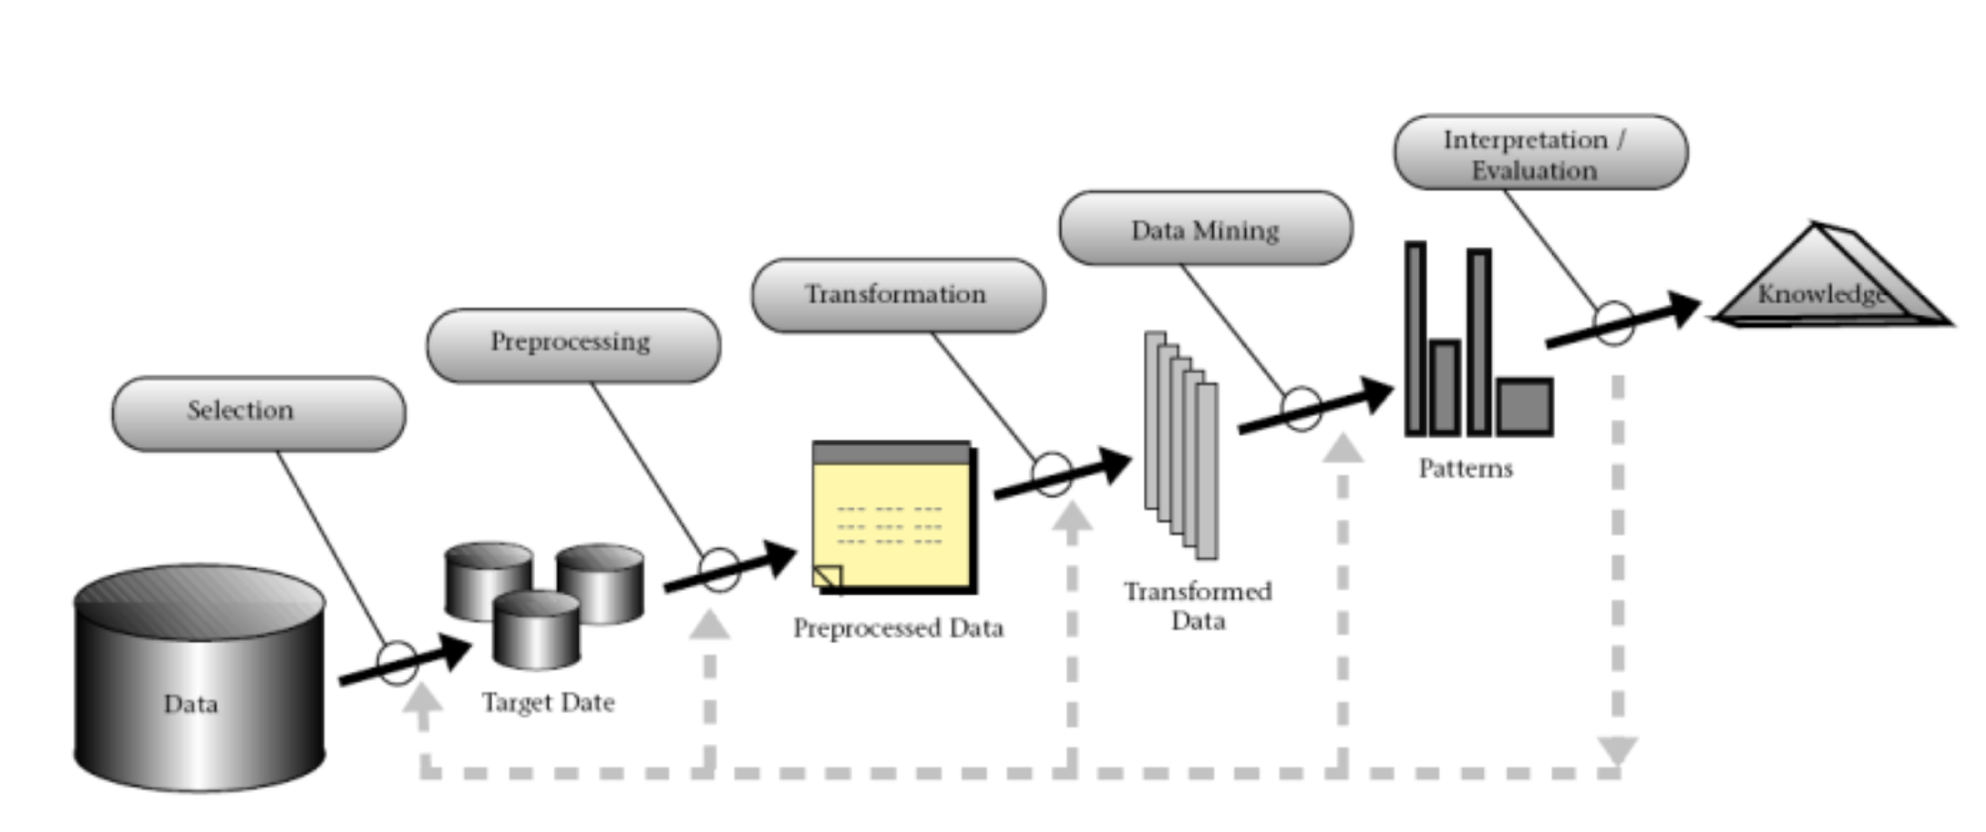
\includegraphics[width=\textwidth]{gfx/kdd.png}
	\caption{Schritte die den KDD Prozess zusammensetzen \cite{FAY:96}}
	\label{fig:process:alt:cor}
\end{figure}

Der Prozess umfasst die nachfolgenden Phasen.
\begin{enumerate}
  \item Selektion (engl.: Selection): \\
  Mit der Selektion soll ein Ziel-Datensatz definiert werden bzw. eine Menge an
  Variablen und Beispiel-Datensätzen festgelegt werden welche zur Feststellung
  neuer Erkenntnisse dienen sollen.
  \item Vorverarbeitung (engl.: Pre processing): \\
  In diesem Schritt sollen die Daten bereinigt werden und dadurch eine gewisse
  Konsistenz gewährleistet werden.
  \item Transformation (engl.: Transformation):
 \\
  Hier sollen durch anwenden verschiedener Transformationen die Daten auf
  wesentliche Einträge (vor allem hinsichtlich ihrer Dimension) reduziert werden.
  \item Data Mining:
 \\
  Mit Data Mining soll nach Mustern innerhalb der Daten gesucht werden und diese
  entsprechend in eine repräsentative Form gebracht werden.
  \item Interpretation / Evaluation:
 \\
  Zuletzt sollen die gefundenen Muster hinsichtlich ihrer Aussagekraft evaluiert werden.
\end{enumerate}

In gewisser Hinsicht kann der KDD Prozess mit dem CRISP-DM Prozess verglichen werden:
\begin{itemize}
  \item Die Phase des „Business Understanding“ (CRISP-DM) korrespondiert mit dem
  Entwickeln eines Verständnisses des Anwendungsgebiets, dem jeweiligen
  Vorwissen und dem festlegen eines Ziels für den Endnutzer (KDD)
  \item Der Schritt „Data Unterstanding“ (CRISP-DM) ist vergleichbar mit einer
  Kombination aus „Selection“ und „Preprocessing“ (KDD)
  \item Die „Data Preparation“ (CRISP-DM) kann identifiziert werden mit der
  „Transformation“ (KDD)
  \item Die „Modeling“ (CRISP-DM) Phase entspricht in etwa dem „Data Mining“ (KDD)
  \item „Evaluation“ (CRISP-DM & KDD) kann gleichgesetzt werden
  \item Letztendlich kann „Deployment“ (CRISP-DM) mit der Konsolidierung (KDD)
  beschrieben werden indem die gewonnenen Erkenntnisse ins System eingebunden
  werden
\end{itemize}

\subsection{Der Data Mining Prozess SEMMA}
\label{sec:process:alt:semma}

Das Akronym SEMMA steht für „Sample Explore Modify Model Assess“ und wurde vom
SAS Institute entwickelt. Auch wenn der Prozess prinzipiell unabhängig vom
gewählten Softwaretool ist, gibt es hier eine Verbindung zur von SAS
bereitgestellten Software „SAS Enterprise Miner“. \\
Die Phasen werden wie folgt beschrieben:
\begin{enumerate}
  \item Probieren (engl.: Sample):
 \\
  In diesem (optionalen) Schritt soll eine Untermenge an Datensätzen ausgewählt
  werden, welche zwar alle Struktur-relevanten Daten beinhaltet allerdings immer
  noch klein genug ist um schnell manipuliert werden zu können.
  \item Entdecken (engl.: Explore): \\
  Hier sollen die Datensätze auf unerwartete Trends und Anomalien untersucht
  werden um ein Verständnis der Daten und der Struktur zu gewinnen.
  \item Modifizieren (engl.: Modify):
 \\
  Durch Modifikation der Daten, also Selektion und Transformation, sollen diese
  so kombiniert werden, sodass ein Mining Model ausgewählt bzw. darauf
  angewendet werden kann.
  \item Modellieren (engl.: Model):
 \\
  Diese Phase soll dazu dienen, die Daten zu modellieren, d.h. mithilfe einer
  entsprechenden Software automatisch nach einer Kombination von Datensätzen zu
  suchen, welche ein gewünschtes Ergebnis vorhersagen.
  \item Beurteilen (engl.: Assess):
 \\
  Zuletzt soll das Ergebnis beurteilt werden, indem die Genauigkeit und
  Nützlichkeit der Funde evaluiert werden und abgeschätzt wird wie effizient der
  Prozess insgesamt ist.
\end{enumerate}
